\title{Vorbis}

\author{Vicente González Ruiz}

\maketitle
\tableofcontents

\section{What is Vorbis?}
%{{{

\begin{itemize}
\item Vorbis~\cite{Vorbis, Vorbis-doc} is a lossy perceptual (psycho
  acoustic) digital audio compressor.
\item The encoder inputs \href{../Digital_Signals/index.html}{PCM (digital)} audio and outputs Ogg
  data.
\begin{center}
\begin{verbatim}
PCM   +---------+  Ogg   +---------+ PCM
----->| Encoder |------->| Decoder |----->
audio +---------+ stream +---------+ audio'

              audio != audio'
\end{verbatim}
\end{center}
\end{itemize}

%}}}

\section{What is Ogg Vorbis?}
%{{{

\begin{itemize}
\item Ogg Vorbis is a:
  \begin{itemize}
  \item fully open, non-proprietary, patent-and-royalty-free,
  \item general-purpose compressed \emph{audio format}
  \item for mid to high quality (8 kHz - 48.0 kHz, 16 bit, polyphonic)
    audio (human voice, e.g.) and music
  \item at fixed and variable bitrates from 30 to 500
    kbps/channel.
  \end{itemize}
\end{itemize}

%}}}

\section{Why Vorbis born?}
%{{{

\begin{itemize}
\item In September 1998 the Fraunhofer Society sends a \href{https://www.chillingeffects.org/patent/notice.cgi?NoticeID=464}{letter of
  infringement} to several small commercial and open source MPEG audio
  layer 3 development projects, announcing plans to charge licensing
  fees for the MP3 audio format.
\item In that moment and for that reason (among others), a company
  named Xiphophorus and founded by Chris Montgomery, starts to develop
  the open-source Vorbis and Ogg projects.
\end{itemize}

%}}}

\section{How Vorbis is used?}
%{{{

\begin{itemize}
\item Unfortunately, the technical information about how Vorbis works
  is quite obscure. However, there is a set of libraries and tools
  \href{http://www.vorbis.com/setup_linux/}{libogg/libvorbis/vorbis-tools}
  that do the hard work for the programmers. The Xiph.org foundation
  maintains these source/binary codes.
\item Several \href{http://www.vorbis.com/software/}{independent
  open-source encoders and players} are also available.
\end{itemize}

%}}}

\section{Who uses Vorbis?}
%{{{

\begin{center}
  \begin{tabular}{|r|r|r|r|}
    \hline
    \href{http://evolver.fm/2013/05/13/spotify-uses-different-audio-formats-depending-on-platform/}{Spotify} &
    \href{http://audacity.sourceforge.net/about/features}{Audacity} &
    \href{http://www.winamp.com/plugin/ogg-vorbis-encoder-v1-1/143936}{WinAmp} &
    \href{http://gstreamer.freedesktop.org/documentation/plugins.html}{GStreamer} \\
    \hline
    \href{http://www.fsf.org/campaigns/playogg/en/}{VLC Media Player} &
    \href{http://en.wikipedia.org/wiki/Use_of_Ogg_formats_in_HTML5}{Firefox} &
    \href{http://en.wikipedia.org/wiki/Use_of_Ogg_formats_in_HTML5}{Chrome} &
    \href{http://en.wikipedia.org/wiki/HTML5_video}{Android} \\
    \hline
    \href{http://www.w3.org/wiki/HTML/Elements/video}{HTML5} &
    &
    &
    \\
    \hline
  \end{tabular}
\end{center}

%}}}

\section{Licensing}
%{{{

\begin{itemize}
\item Vorbis is used under the BSD (Berkeley Software Distribution) license, which basically means:
\begin{enumerate}
\item You can use the source code to develop new open source BSD
  applications and
\item you can use the source code to develop propietary applications.
\end{enumerate}
\end{itemize}

%}}}

%}}}


\section{The Vorbis encoder}
%{{{

\begin{center}
\begin{verbatim}
          PCM   +---------+  Ogg
          ----->| Encoder |------->
          audio +---------+ stream
               /           \
            /                 \
         /                       \
     /                               \
 /                                       \
+--------+    +-----+    +---+    +-------+
| W+MDCT |--->| SAM |--->| Q |--->| VQ+HE |
+--------+    +-----+    +---+    +-------+

W+MDCT = Windowed Modified Discrete Cosine Transform
SAM = pSycho Acoustic Model
Q = Quantization
VQ+HE = Vector Quantization + Huffman Encoding
\end{verbatim}
\end{center}

%}}}

\section{Overlaped processing}
%{{{

Uses \href{https://en.wikipedia.org/wiki/Modified_discrete_cosine_transform}{MFCT}.

\begin{center}
\begin{verbatim}
0              N-1            2N-1            3N-1
+---------------+---------------+---------------+ s[n]
<--------Transform Step--------->
                <---------Transform Step-------->
\end{verbatim}
\end{center}

\begin{itemize}
\item Each transform step inputs $2N$ samples and outputs $N$ MDCT
  coeficients.
\item $N$ can vary depending on the characteristics of the sound. For
  \emph{complex} sounds without clear armonics (such as a plosive
  sound), shortened windows improve the performance. For \emph{simple}
  sounds (such as a music instrument), large windows are better.
\item The window size ($N$) must me a power of two between 64 and 8192
  samples.
\end{itemize}

%}}}

\section{MDCT (Modified Discrete Cosine Transform)}
\begin{itemize}
\item Equivalent to apply a
  \href{http://en.wikipedia.org/wiki/Filter_bank}{bank} of $N$
  filters.
\item Determines the correlation between a set of $2N$ numbers
  (samples) and $N$
  \href{http://en.wikipedia.org/wiki/Orthogonality}{orthogonal}\footnote{Two
    functions/signals are orthogonal if it is impossible to obtain one
    of them by means of the other.}
  \href{http://guru.multimedia.cx/mdct/}{cosine functions}. Therefore,
  at the input of the DCT there are $2N$ samples and at the output,
  $N$ coefficients.
\item The MDCT coefficients $S[w]$ of the PCM samples $s[n]$ are
  defined as:
\begin{equation}
  S[w] =
  \sum_{n=0}^{2N-1}s[n]cos\Big[\frac{\pi}{N}(n+\frac{1}{2}+\frac{N}{2})(w+\frac{1}{2})\B
    ig].
  \label{eq:MDCT}
\end{equation}

\section{Windowing}
%{{{

\begin{itemize}
\item Samples are windowed before the transform because this acurates
  the spectral energy estimation\footnote{The spectrum of finite
    sequences is the spectrum of the convolution of the spectrum of
    the sequence with the spectrum of the windowing function, so, the
    narrower the spectrum of the windowing function, the accurater the
    computed spectrum of the finite sequence}:
\end{itemize}

\begin{center}
\ifx \HCode\Undef

  \begin{tabular}{cc}
    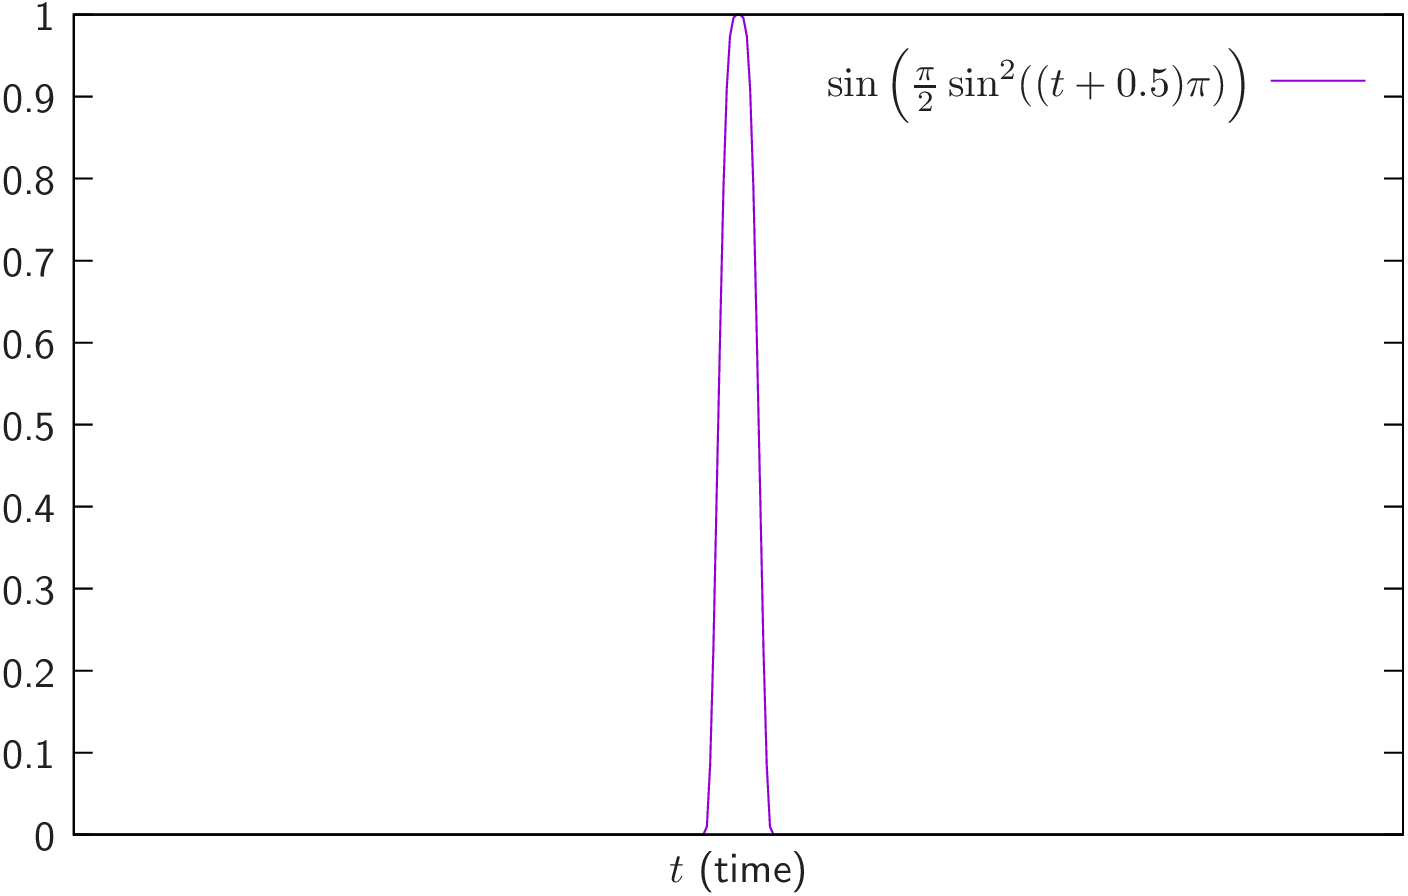
\includegraphics[width=0.45\textwidth]{window} &
    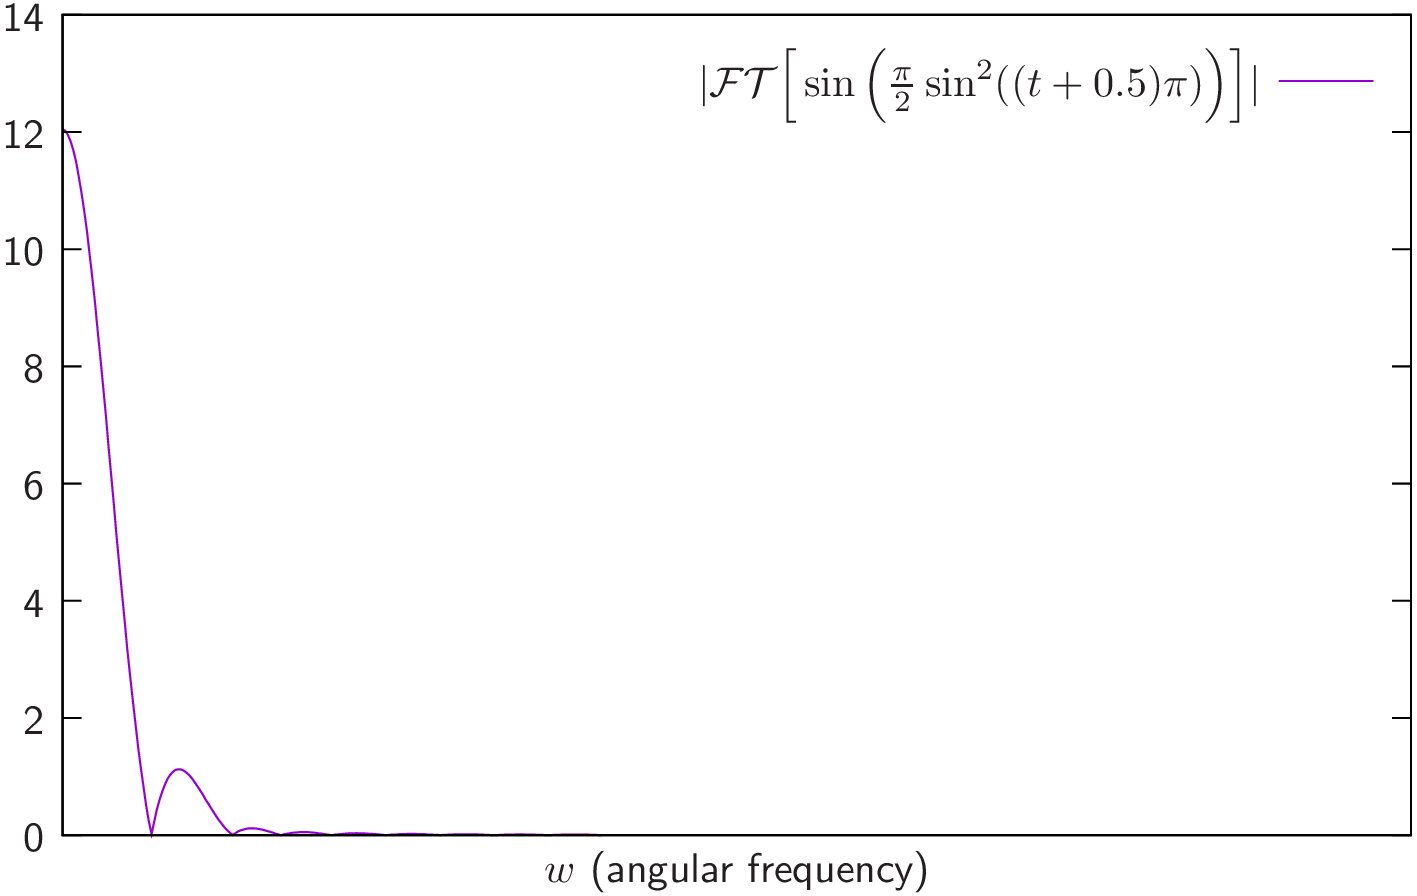
\includegraphics[width=0.45\textwidth]{window_spectrum}
  \end{tabular}

\else

  \begin{tabular}{c}
    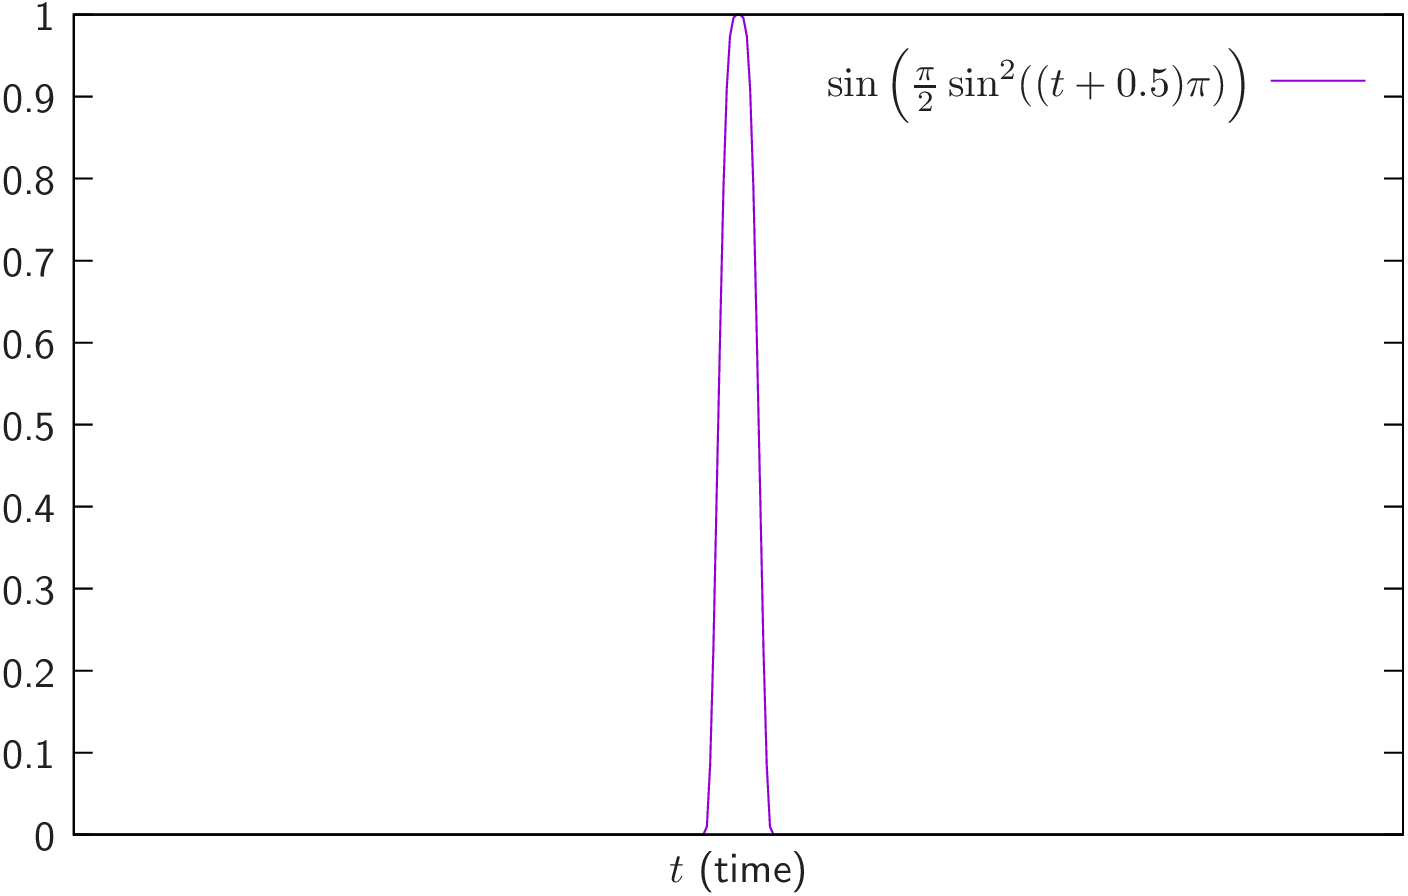
\includegraphics[width=0.45\textwidth]{window} \\
    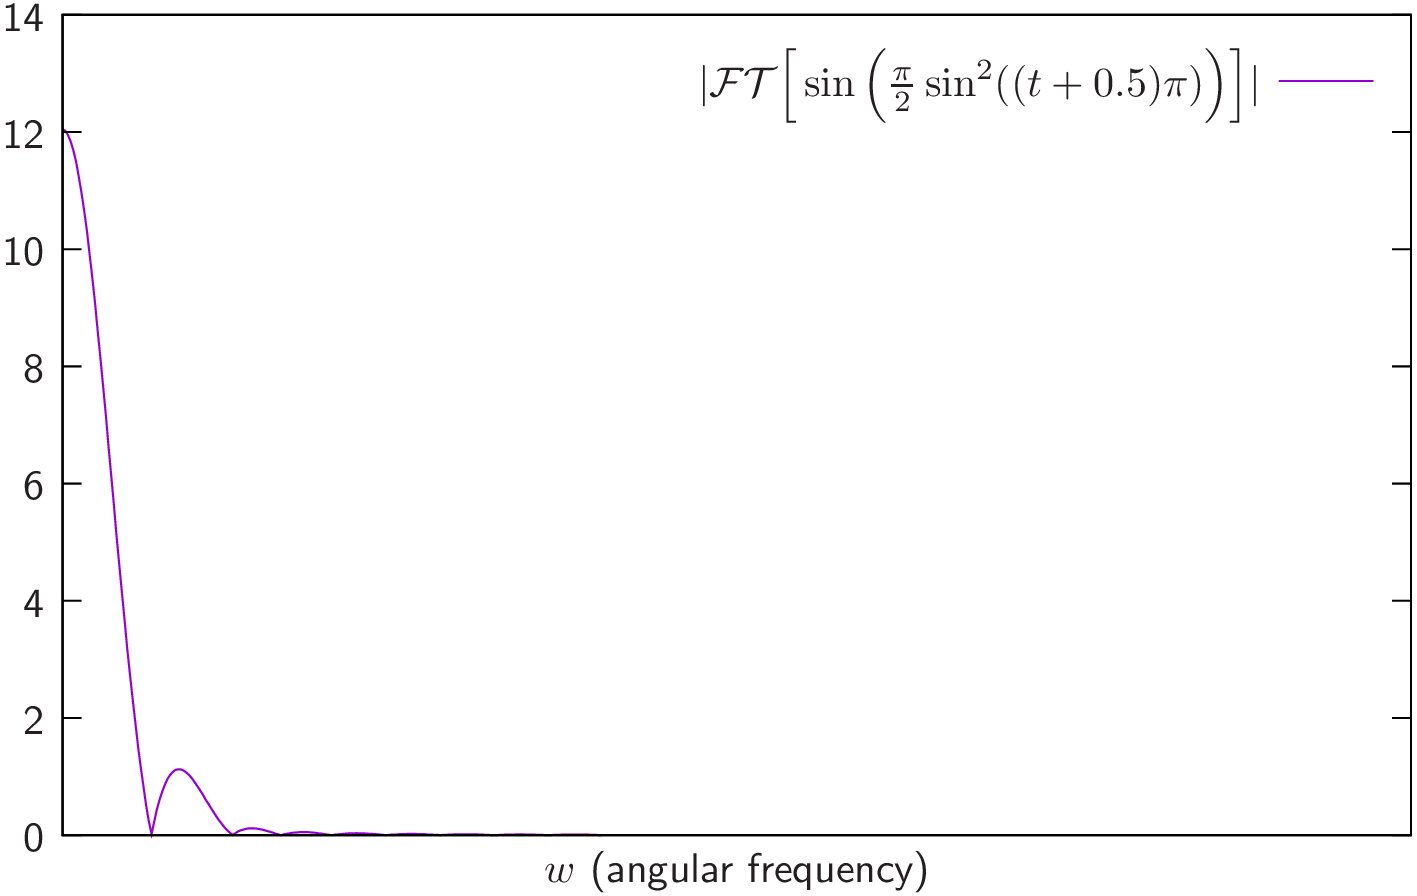
\includegraphics[width=0.45\textwidth]{window_spectrum}
  \end{tabular}
\fi
\end{center}

%}}}

\section{Quantization}
%{{{

\begin{itemize}
\item These are the quantization levels available for Vorbis:
  \begin{center}
    \begin{tabular}{r|l}
      Quality & Expected bit-rate (Kbps) \\
      \hline
      -2 & 32 \\
      -1 & 45 \\
      0 & 64 \\
      1 & 80 \\
      2 & 96 \\
      3 & 112 \\
      4 & 128 \\
      5 & 160 \\
      6 & 192 \\
      7 & 224 \\
      8 & 256 \\
      9 & 320 \\
      10 & 500
    \end{tabular}
  \end{center}
%\item Notice that the ATH model says that the quantization steps
%  should depend on the bark (the step should be smaller in central
%  frequencies).
%\item The quantization creates a quantization-noise signal in each bark.
%\item Inside of a bark (and taking into account the temporal masking),
%  those tones that are 4dB below of the quantization noise are
%  imperceptible for the most part of the audience, and can be ignored.
%\item As a result, the frequency information can be encoded with a
%  lower bit-rate.
\end{itemize}

%}}}

\section{Floor and residue encoding}
%{{{

\begin{itemize}
\item The quantized frequency spectrum is approximated with a
  polynomial (the floor curve). This curve is lossless encoded and has
  much less data (coefficients) and information than the quantized
  spectrum.
\item The difference (residue) between the floor curve and the
  quantized spectrum is
  \href{http://www.data-compression.com/vq.shtml}{VQ}+\href{../Text_Coding/index.html#x1-6900015}{Huffman}
  (lossy) encoded.
\end{itemize}

%}}}

\section{Vorbis's VQ (Vector Quantization)}
%{{{

\begin{itemize}
\item Embedded (truncable) CBR (Constant Bit-Rate) lossy encoding.
\item Minimize quantization error when tuples of symbols are encoded.
\begin{center}
\begin{verbatim}
 tuples  +---------+ code-vectors
-------->| Encoder |--------->
         +---------+
\end{verbatim}
\end{center}
\item A output code-vector is the index of the tuple in the codebook
  (the set of code-vectors) that is most similar to the input tuple.
\item In Vorbis, the code-book is computed for each audio sequence.
\end{itemize}

%}}}

\section{Huffman coding}
%{{{

\begin{itemize}
\item Variable bit-rate (VBR) lossless encoder.
\item The Huffman codes are computed using the probabilities of the
  code-vectors, floor coefficients, etc.
\item This lossless stage increase the compression ratio of the
  spectral residues.
\end{itemize}

%}}}

\section{Packet ``peeling''}
\begin{itemize}
\item Because the order in which the infomation is written into a
  Vorbis packet (firt the floor data and next the residue data), these
  can be truncated in order to reduce the bit-rate, without
  re-encoding.
\end{itemize}

\section{Channel coupling}
%{{{

\begin{itemize}
\item Vorbis supports up to 255 channels.
\item Most of times, similar sounds are transported in several
  channels.
\item Channel coupling decreases inter-channel redundancy.
\item Residue spectrums of mutichannel audios tend to be correlated.
%\item In Vorbis, the differences between these residue spectrums are
%  mapped in a square/polar representation (similar to a module/phase
%  represention of a vector). After this, and depending on the quality
%  parameter, three coupling methods can be used:
\item The differences between these residue spectrums are coded using
  one of the following methods:
  \begin{enumerate}
  \item \textbf{Lossless coupling:} All stereo information
    (differences between left and right samples) is lossless
    compressed. This provides the maximal quality but the minimal
    compression.
  \item \textbf{Phase stereo:} Stereo information is quantized and
    compressed. Sterie information is represented in a square polar
    representation (module and phase) and phase is quantized.
  \item \textbf{Point stereo:} All polar (stereo) information is
    discarded. In this case, all the stereo information comes from the
    difference in the spectral floors for the channels. This provides
    the maximal compression but the minimal quality.
  \end{enumerate}
\end{itemize}

%}}}

\section{Perceptual quantization & white-noise filling}

\begin{itemize}
\item Depending on the desired output bit-rate and the frequency (see
  the ATH model), the SAM applies a different quantization step to
  barks. Roughly speaking, the higher the compression ratio, the
  larger the quantization step and therefore, the quantization noise;
  and the higher the frequency, the wider the bark. Notice also that
  the perception of a tone in a bark depends also on the temporal
  masking.
\item At decoding time, those barks that suffered the biggest lossess
  are usually filled with
  \href{http://en.wikipedia.org/wiki/White_noise}{white noise} in
  order to \href{http://simplynoise.com/}{increase the perceived
    quality}.
\end{itemize}


\section{What is Ogg?}
%{{{

\begin{itemize}
\item A free, open container format maintained by the Xiph.Org
  Foundation.
\item It can multiplex a number of independent streams for audio,
  video, text (such as subtitles), and metadata.
\end{itemize}

%}}}

\section{The Ogg format}
%{{{

\fig{400}{Ogg_Stream.png}

\begin{itemize}
\item In a Ogg Vorbis stream, the first pages store a header with the
  information neccesary to decode the rest os pages (e.g. the
  code-book and the Huffman tree). The rest of pages store audio.
\end{itemize}

%}}}

\bibliography{Vorbis}
